
\cleardoublepage


\chapter{Experimental Validation}



\section{Postprocessing and Results}


\subsection{Gold Foil Tube}


% postprocessing includes taking the measured activities and converting them to saturation activities
The postprocessing necessary for a foil activation experiment involves taking the measured activities, which are reported from the gamma spectrometry software, and backing out the saturation activities for each foil.
% this is done using the following equation
This is done using the following equation,

% how to get saturation activities
\begin{equation}
\label{eqn:a_sat}
A_{sat} = A_{meas} \frac{R_{meas}}{R_{sat} n_a K I_{rel}} ,
\end{equation}

% where, (explain these terms)
where $R_{meas}$ is the ratio that corrects for decay during measurement, $R_{sat}$ is the saturation ratio which will be explained below, $n_a$ is the number of sample atoms, equal to $\rho N_A / M$, $K$ is the isotopic abundance, and $I_{rel}$ is the relative intensity of the counted gamma ray.

% give the term and explain for r_meas
The term, $R_{meas}$ is the ratio of the activity at the beginning of the gamma counting to the activity assuming the decay is constant during counting.
It is given by the following equation

% measurement ratio/correction factor
\begin{equation}
\label{eqn:r_meas}
R_{meas} = \frac{\lambda t_{meas}}{1 - e^{\lambda t_{meas}}},
\end{equation}

in which $\lambda$ is the decay constant and $t_{meas}$ is the time during measurement.

% explain the concept of saturation ratio
The saturation ratio, $R_{sat}$, is the ratio between the activity at the time of measurement and the saturation activity.
Although this value generally assumes constant production during irradiation followed by a period of decay with no production, a method has been developed that captures transient behavior in reactor fluxes which will be detailed here.

The production and decay of radioisotopes is expressed mathematically through the bateman equation,

\begin{equation}
\label{eqn:bateman}
\frac{dN(t)}{dt} = C(t) - \lambda N(t)
\end{equation}

where $N(t)$ is the number of radioactive nuclei in the sample, C(t) is the production term in nuclei per second, and $\lambda$ is the decay constant for the isotope in consideration.
The change in radionuclei is simply the production minus the loss.
The relationship between activity and radionuclides, $A(t) = \lambda N(t)$ allows us to convert \EQ{eqn:bateman} into the following,

\begin{equation}
\label{eqn:bateman_activity}
\frac{A(t)}{dt} = \lambda (C(t) - A(t)).
\end{equation}

We can then divide each of the terms by $C_{sat}$ which is the isotopic production at nominal power.
This value is equal to the saturation activity, since the activity at $t = \inf$ for nominal power is equal to the production at that power.

\begin{equation}
\label{eqn:bateman_ratios}
\frac{A(t) / C_{sat}}{dt} = \lambda (\frac{C(t)}{C_{sat}} - \frac{A(t)}{C_{sat}})
\end{equation}

Two facts allow us to simplify \EQ{eqn:bateman_ratios} into a useful form.
First, because $A_{sat} = C_{sat}$, any $A(t) / C_{sat} = A(t) / A_{sat}$, so we can replace these terms with a defined term, $R_{sat}(t)$ which is the ratio of the activity at time $t$ to the saturation activity.
Second, although we don't have access to the $C(t)$ or $C_{sat}$ terms since they require the (currently unknown) flux, we do have access to power data.
Because isotopic production is approximately proportional to reactor power, $C(t) \propto P(t)$, this means that $C(t) / C_{sat} \approx P(t) / P_{nominal}$.
We will replace this power ratio with the term $P_{f}(t)$, which is simply the time dependent ratio of the power to the nominal power.

\begin{equation}
\label{eqn:bateman_r_sat}
\frac{R_{sat}(t)}{dt} = \lambda (P_{f}(t) - R_{sat}(t))
\end{equation}

This equation can be solved to find $R_{sat}$ at the time of measurement using a numerical solver, in our case, {\tt scipy}'s {\tt odeint}.
The data for $P_{f}(t)$ is simply normalized strip chart data collected from an in-core fission chamber.


% ---------------------
% fix this table later
% ---------------------

% this contains all of the correction factors and foil activities
\begin{table}[h]\centering
\label{tab:a_sat}
\caption{The correction factors and foil activities.}
\begin{tabular}{ r | r | r | l | r }
\toprule
Position (in.)  & $A_{meas}$ (Bq) & $R_{meas}$  & $R_{sat}$   &   $A_{sat}$  (Bq)\\
0 & 1483.73 & 1.00089 & 0.02268 & 65468.28 \\
1 & 58.60 & 1.00590 & 0.02262 &  2605.89  \\
2 & 8.92 & 1.03805 & 0.02196 &   422.02  \\
3 & 4.06 & 1.06581 & 0.0204  &   212.01  \\
4 & 2.58 & 1.14023 & 0.01574  &   186.96  \\
5 & 1.60 & 1.27976 & 0.01340 &      153.12  \\
6 & 0.72 & 1.26894 & 0.00794 &       115.22  \\
7 & 0.37 & 1.27340 & 0.00483 &      97.03   \\
8 & 0.17 & 1.41587 & 0.00256 &       95.65\\
\end{tabular}
\end{table}

% foil responses
\begin{figure}[htb]
\centering
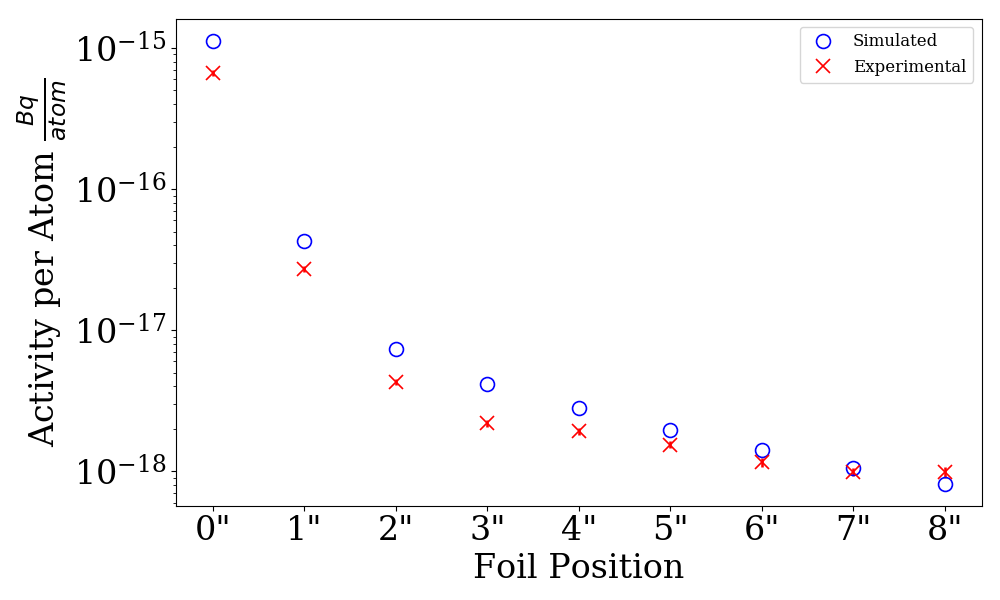
\includegraphics[height=3in]{tex/figures/compare_activities.png}
\caption[Foil Activities]{A comparison of the simulated and experimentally obtained foil activities.}
\label{fig:compare_activities}
\end{figure}


\subsection{Bonner Sphere Spectrometer}

The BSS data was processed simply by taking the area under the LiI reaction peaks and dividing that value by the live time of the detector.
These values are presented in \TAB{tab:bss}.

% bss response integration
\begin{figure}[htb]
\centering
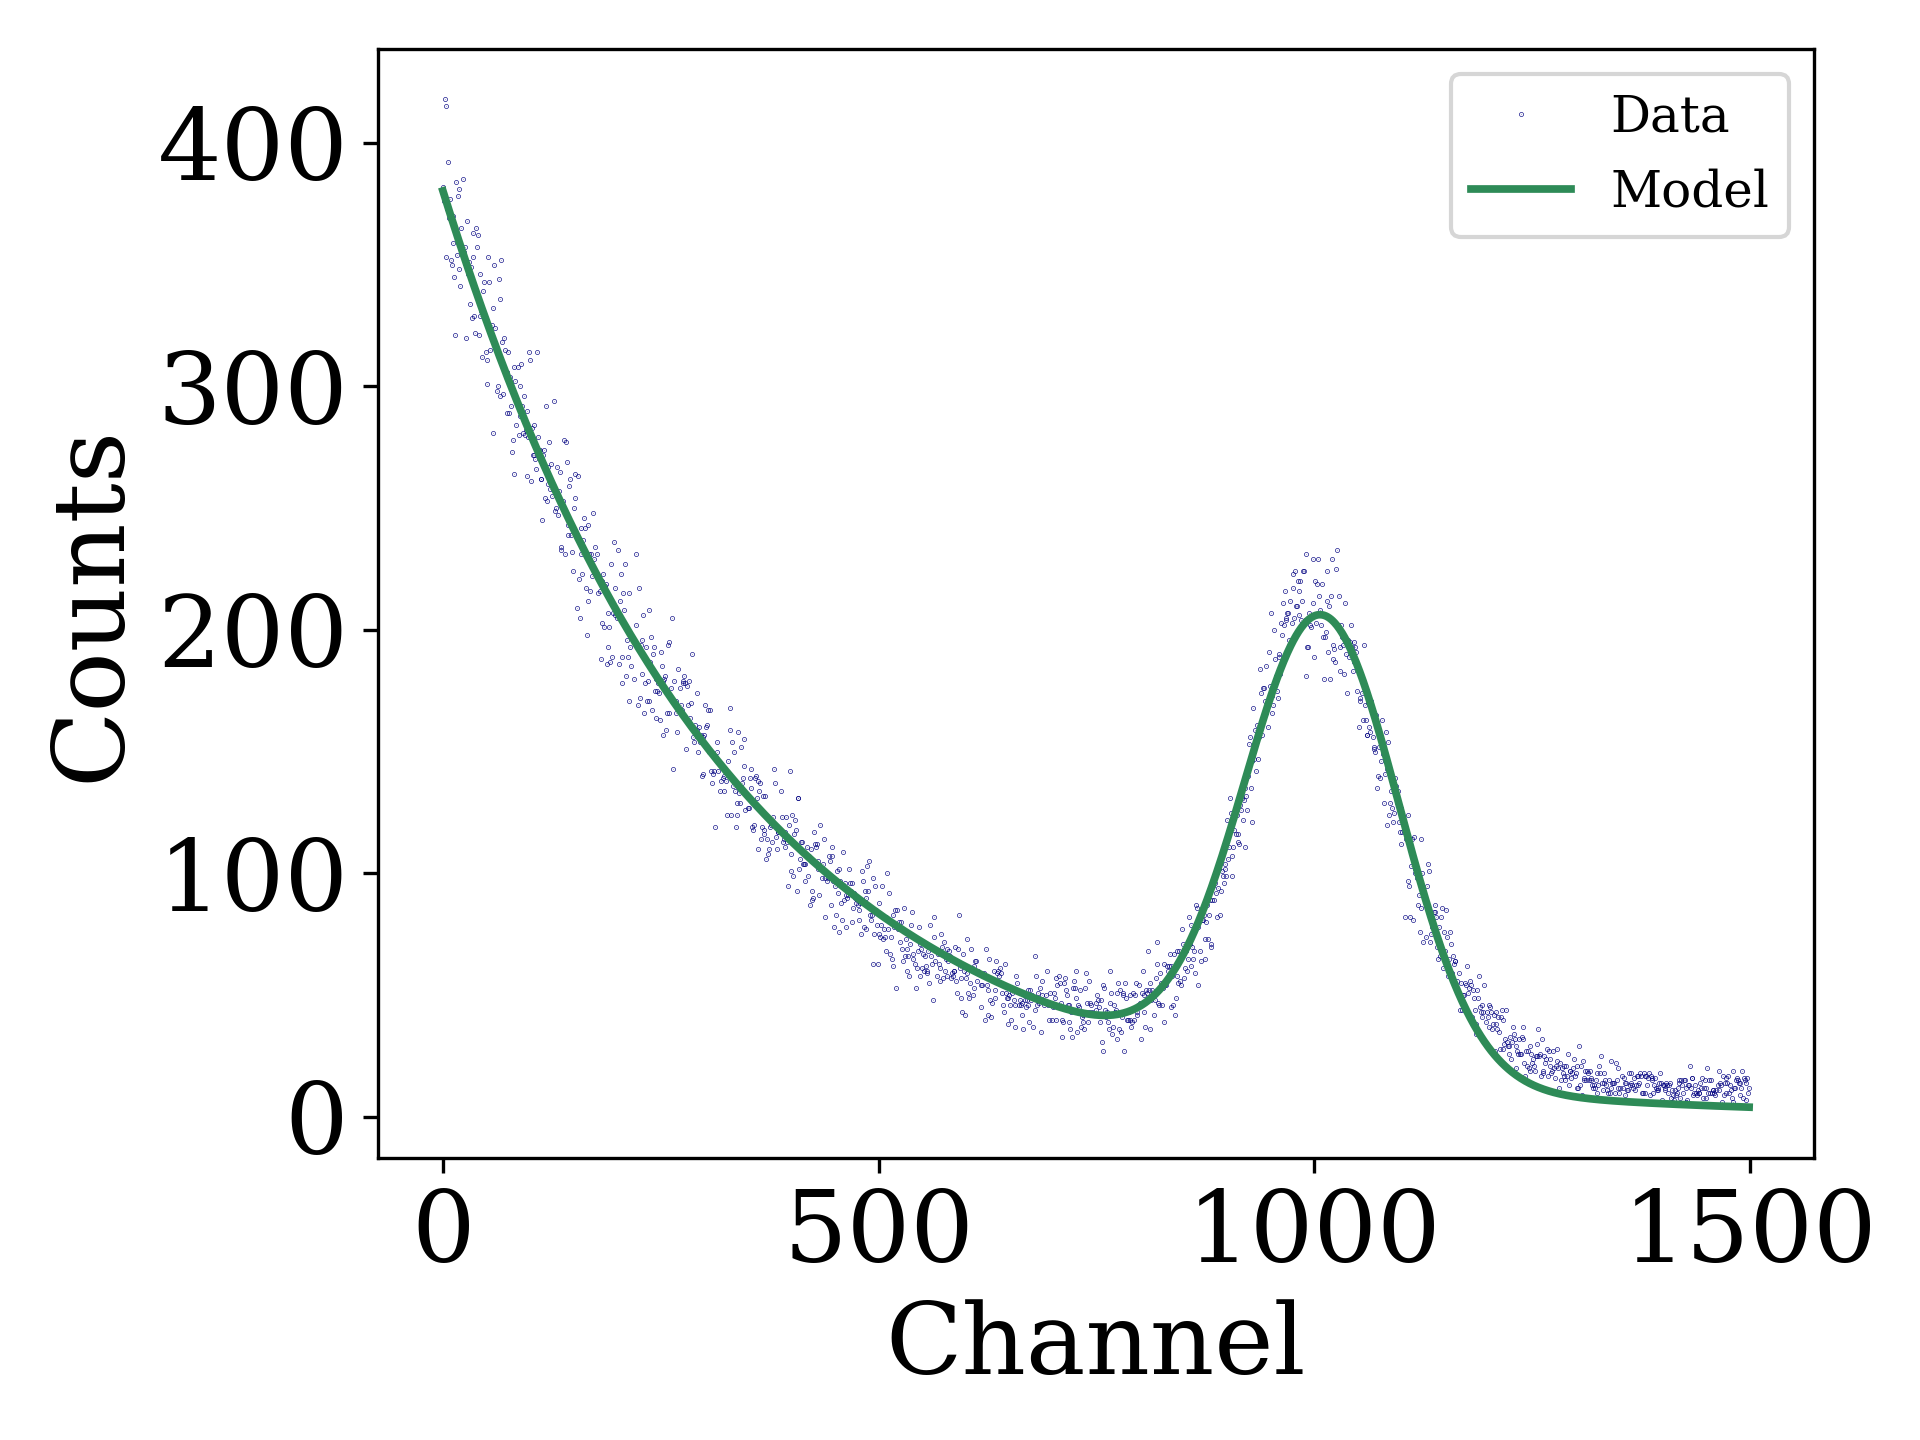
\includegraphics[height=3in]{tex/figures/bs4_spectrum.png}
\caption[8" BSS Spectrum]{The 8" sphere's gamma-ray spectrum and the model used to find the integral response.}
\label{fig:compare_countrates}
\end{figure}


% the bss count rates
\begin{table}[h]\centering
\label{tab:bss}
\caption{The BSS count rates from the experiment.}
\begin{tabular}{ r | r }
\toprule
Sphere (in.)  & Count Rate $s^{-1}$\\
Bare & 1626.76\\
2  & 1062.40\\
3 & 3891.13\\
5 & 417.24\\
8 & 139.72\\
10 & 70.75\\
12 & 37.43\\
\end{tabular}
\end{table}

% bss responses
\begin{figure}[htb]
\centering
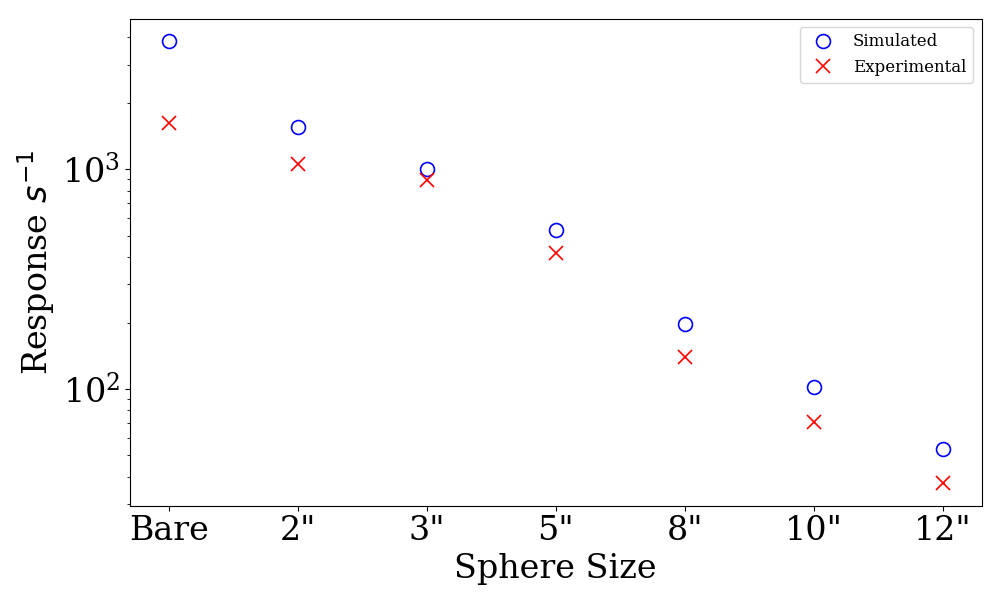
\includegraphics[height=3in]{tex/figures/compare_countrates.png}
\caption[BSS Responses]{A comparison of the simulated and experimentally obtained BSS responses.}
\label{fig:compare_countrates}
\end{figure}



